\newcommand{\instFun}[2]{\texttt{#1}\ensuremath{_{#2}}\xspace}

\section{GRE via Building Simulated Models}\label{sec:krahmer}

Krahmer~et~al.~\cite{Krahmer2003} introduce an algorithm for
content determination based on the computation of \emph{subgraph isomorphisms}.
It is heavily regulated by cost functions and is therefore apt to implement
different preferences. In fact, they show that using suitable cost functions it
can simulate most of the previous proposals. Their algorithm takes as input
a labeled directed graph $G$ and a node $e$ and returns, if possible,
a connected subgraph $H$ of $G$, containing $e$ and enough edges to
distinguish $e$ from the other nodes.

In this section we will identify its
underlying notion of expressiveness and  will extend it to accommodate other notions.
To keep the terminology of~\cite{Krahmer2003}, in what follows
we may alternatively talk of \emph{labeled graphs} instead of relational
models. The reader should observe that they are essentially the same
mathematical object, but notice that in~\cite{Krahmer2003},  propositions are encoded using
looping binary relations (e.g., they write $\nDog(e,e)$ instead of $\nDog(e)$).

The main ideas of their algorithm can be
intuitively summarized as follows.
Given two labeled graphs $H$ and $G$, and vertices $v$ of $H$
and $w$ of $G$, we say that the pair $(v,H)$ {\em refers}
to the pair $(w,G)$ iff $H$ is connected and $H$ can be ``placed
over'' $G$ in such a way that: 1) $v$ is placed over $w$; 2) each
node of $H$ is placed over a node of $G$ with at least the same
unary predicates (but perhaps more); and 3) each edge from $H$ is
placed over an edge with the same label. Furthermore, $(v,H)$ {\em
uniquely refers} to $(w,G)$ if $(v,H)$ refers to $(w,G)$ and there
is no vertex $w'\not=w$ in $G$ such that $(v,H)$ refers to $(w',G)$.
The formal notion of a labeled graph being ``placed over'' another
one is that of {\em subgraph isomorphism}:
$H=\tup{\Delta_H,\interp{\cdot}_H}$ can be placed over
$G$ iff there is a labeled subgraph (i.e., a graph obtained from
$G$ by possibly deleting certain nodes, edges, and propositions from some nodes)
$G'=\tup{\Delta_{G'},\interp{\cdot}_{G'}}$ of $G$ such that $H$ is {\em
isomorphic} to $G'$, which means that there is a
bijection $f:\Delta_{H}\to\Delta_{G'}$ such that for all vertices
$u,v\in \Delta_H$, $u\in\interp{p}_{H}$ iff $f(u)\in\interp{p}_{G'}$
and $(u,v)\in\interp{r}_{H}$ iff $(f(u),f(v))\in\interp{r}_{G'}$.
%
\begin{figure}
\centering
\begin{tabular}{c@{\hspace{1.0cm}}c@{\hspace{1.0cm}}c@{\hspace{1.0cm}}c}
\begin{picture}(22,50)
\put(0,0){\begin{tikzpicture}
  [
    n/.style={circle,fill,draw,inner sep=1.5pt,node distance=1.5cm},
    aSniffing/.style={->, >=stealth, semithick, shorten <= 3pt, shorten >= 3pt},
  ]
 \node[n,label=above:$v$,label=below:{\relsize{-1}$\begin{array}{c}\nDog\\\ \end{array}$}] (a) {};
 \end{tikzpicture}}
 \end{picture}
&
\begin{picture}(55,50)
\put(0,0){\begin{tikzpicture}
  [
    n/.style={circle,fill,draw,inner sep=1.5pt,node distance=1.5cm},
    aSniffing/.style={->, >=stealth, semithick, shorten <= 3pt, shorten >= 3pt},
  ]
 \node[n,label=above:,label=below:{\relsize{-1}$\begin{array}{c}\ \end{array}$}] (a) {};

 \node[n,label=above:$v$,label=below:{\relsize{-1}$\begin{array}{c}\nDog\\\ \end{array}$}, right of=a] (b) {};

 \draw [aSniffing,bend right=40] (b) to node[auto,swap]{\relsize{-1}$\aSniffing$} (a);

 \end{tikzpicture}}
 \end{picture}
&
\begin{picture}(70,50) \put(0,0){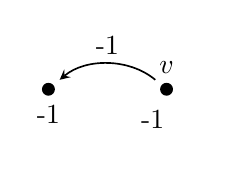
\begin{tikzpicture}
  [
    n/.style={circle,fill,draw,inner sep=1.5pt,node distance=1.5cm},
    aSniffing/.style={->, >=stealth, semithick, shorten <= 3pt, shorten >= 3pt},
  ]
 \node[n,label=above:,label=below:{\relsize{-1}$\begin{array}{c}\nDog\end{array}$}] (a) {};

 \node[n,label=above:$v$,label=below:{\relsize{-1}$\begin{array}{c}\nDog\\ \aSmall \end{array}$}, right of=a] (b) {};

 \draw [aSniffing,bend right=40] (b) to node[auto,swap]{\relsize{-1}$\aSniffing$} (a);

 \end{tikzpicture}}
 \end{picture}
&
\begin{picture}(77,50)
\put(0,0){\begin{tikzpicture}
  [
    n/.style={circle,fill,draw,inner sep=1.5pt,node distance=1.5cm},
    aSniffing/.style={->, >=stealth, semithick, shorten <= 3pt, shorten >= 3pt},
  ]
 \node[n,label=above:$v$,label=below:{\relsize{-1}$\begin{array}{c}\nDog\end{array}$}, right of=a] (b) {};
%
 \node[n,label=above:,label=below:{\relsize{-1}$\begin{array}{c}\nCat\\ \aSmall\end{array}$}, right of=b] (c) {};
%
 \draw [aSniffing,bend right=40] (c) to node[auto,swap]{\relsize{-1}$\aSniffing$} (b);
 \end{tikzpicture}}
 \end{picture}
% %
% \begin{picture}(77,50)
% \put(0,0){\begin{tikzpicture}
%   [
%     n/.style={circle,fill,draw,inner sep=1.5pt,node distance=1.5cm},
%     aSniffing/.style={->, >=stealth, semithick, shorten <= 3pt, shorten >= 3pt},
%   ]
%  \node[n,label=above:,label=below:{\relsize{-1}$\begin{array}{c}\end{array}$}] (a) {};
%
%  \node[n,label=above:$v$,label=below:{\relsize{-1}$\begin{array}{c}\end{array}$}, right of=a] (b) {};
%
%  \draw [aSniffing,loop left] (a) to node[above,xshift=-5pt]{\relsize{-1}$\aSniffing$} (a);
%
%  \draw [aSniffing,bend right=40] (b) to node[auto,swap]{\relsize{-1}$\aSniffing$} (a);
%  \end{tikzpicture}}
%  \end{picture}
\vspace{-.2cm}\ \\
(i)&(ii)&(iii)&(iv)
\end{tabular}
 \caption{Some connected subgraphs $(v,H)$ of scene $\+S$ in Figure~\ref{fig:cat-dog-1}.\label{fig:subgraphs}}
 \end{figure}

As an example, consider the relational model depicted in
Figure~\ref{fig:cat-dog-1} as a labeled graph $G$, and let us
discuss the pairs of nodes and connected subgraphs $(v,H)$ shown in
Figure~\ref{fig:subgraphs}. Clearly, (i) refers to the pair $(w,G)$
for any node $w\in\{a,b,d\}$; (ii) refers to $(w,G)$ for
$w\in\{b,d\}$; and both (iii) and (iv) uniquely refer to $(b,G)$. Notice
that (i)--(iv) can be respectively realized as ``{\em a dog}'',
``{\em a dog that sniffs something}'', ``{\em a small dog that
sniffs a dog}'' (cf. $\gamma_1$ in Table~\ref{tab:gammas}) % and ``{\em
% something that
% sniffs something else that sniffs itself}''.
and ``{\em the dog that is sniffed by a small cat}'' (cf.~$\gamma_4$ in
Table~\ref{tab:gammas}).


% For reasons of space we assume the reader is familiar with this
% algorithm and refer her to that article for further
% information.\fxnote{\tiny Intentemos depender lo menos posible del
% articulo de Krahmer.  En todo caso, dar una idea intuitiva del
% approach antes de decir esto.  Tenemos todavia una pagina. }



% \fxnote{\tiny Reescribir los siguientes dos parrafos. Decir algo como, 'once
% more we'll try to remain as close as possible to the algorithms of the original
% article and we will then start by pointing out the differences with the algorithms
% we presented in the previous section'}

It is important to emphasize that there is a substantial difference
between the algorithm presented in~\cite{Krahmer2003} and the one we discussed
in the previous sections:
%
% First note that scenes are encoded in that article in a slightly
% different way: there, graphs have only labels on edges, and
% non-relational attributes such as \emph{type} or \emph{color} are
% represented by loops (e.g., $\aSmall(a,a)$). % \fxnote{\tiny Aca decia
% `While our presentation is, arguably, conceptually cleaner, it
% forces us to treat the atomic and relational cases separately'. No
% hablemos de `our presenation' respecto de la de la seccion anterior.
% O ninguna o las dos son `our presentation'. }
%
while the input is a labeled graph $G$ and a target node $v$, the
output is, in this case (and unlike the definition of $\+L$-GRE problem
presented in \sect{technical} where the output is a {\em formula}), the cheapest (with
respect to some, previously specified cost function) connected
{\em subgraph} $H$ of $G$ which uniquely refers to $(v,G)$ if there is
such $H$, and $\bot$ otherwise.

We will not deal with cost functions here; it is enough to know
that a cost function is a monotonic function that assigns to each
subgraph of a scene graph a non-negative number which expresses the
goodness of a subgraph --e.g.\ in Figure~\ref{fig:subgraphs}, one
may tune the cost function so that (iii) is cheaper than (iv), and hence
(iii) will be preferred over (iv).
%By defining cost functions in
%different ways, \cite{Krahmer2003} shows that it is possible to mimic various algorithms for the
%generation of referring expressions known from the literature.

For reasons of space we will not introduce here the detailed algorithm proposed
in~\cite{Krahmer2003}. Roughly, it is a
straightforward branch and bound algorithm that systematically tries all
relevant subgraphs $H$ of $G$ by starting with the subgraph
containing only vertex $v$ and expanding it recursively by trying to
add edges from $G$ that are adjacent to the subgraph $H$ constructed
up to that point. In the terminology
of~\cite{Krahmer2003} a {\em distractor} is a node of $G$ different from
$v$ that is also referred by $H$.
The algorithm ensures that a subgraph uniquely refers to the
target $v$ when it has no distractors. Reached this point we
have a new candidate for the solution, but there can be other
cheaper solution so the search process continues until the
cheapest solution is detected. Cost functions are used to
guide the search process and to give preference to some solutions
over others.
% In the definition of~\cite{Krahmer2003}, $H$ is  such that every \emph{subgraph isomorphism}
% $f$ between $H$ and $G$ (i.e., every isomorphism between $H$
%  and a subgraph of $G$)
%  satisfies $f(u) = u$.
%

Here is the key link between the graph-based method
of~\cite{Krahmer2003} and our logical-oriented perspective: on
finite relational models, subgraph isomorphism corresponds to
\EPFOL-simulations, in the sense that given two nodes $u,v$ of
$G$, there is a subgraph isomorphic to $G$ via $f$, containing $u$ and
$v$, and such that $f(u)=v$ iff $u \simul{\+\EPFOL} v$.
%
Having made explicit this notion of sameness and, with it, the
logical language associated to it, we can proceed to generalize the
algorithm to make it work for other languages, and to adapt it in
order to output a formula instead of a graph. This is shown in
Algorithms~\ref{alg:makeRE} and~\ref{alg:find}.
%
\begin{center}\begin{minipage}[t]{5.1cm}%
\begin{algorithm}[H]\small
\SetKwFunction{makeRE}{makeRE$_\+L$}
\SetKwFunction{findGraph}{find$_\+L$}
\SetKwFunction{init}{init_$\+L$}
\SetKwFunction{buildF}{buildF$_\+L$}

\caption{\small \texttt{makeRE}$_\+L$($v$)}\label{alg:makeRE}

%$v_H$ := \emph{new node}\;

\SetKwInOut{Input}{input}\SetKwInOut{Output}{output}
\Input{an implicit finite $G=\tup{\Delta_G,\interp{\cdot}}$ and $v\in\Delta_G$}
\Output{an $\+L$-RE for $v$ in $G$ if there is one, or else $\bot$}
\BlankLine

\vspace{3.0pt}

\BlankLine

$H$ := $\tup{\cset{v},\emptyset}$\; $f$ := $\cset{v \mapsto v}$\;
$H'$ := \findGraph($v, \bot, H, f$)\;
\BlankLine
\Return{\buildF$(H',v)$}\;
\end{algorithm}
  \end{minipage}
\hspace{.05cm}
  \begin{minipage}[t]{6.8cm}%
\begin{algorithm}[H] \small
\SetKwFunction{findGraph}{find$_\+L$} \SetKwFunction{cost}{cost}
\SetKwFunction{matchGraph}{match$_\+L$}
\SetKwFunction{extendGraph}{extend$_\+L$}


\caption{\small \texttt{find}$_\+L$($v, \mathit{best},
H,f$)}\label{alg:find}

\If{$\mathit{best} \neq \bot \land \cost(\mathit{best}) \leq
\cost(H)$}{\Return $\mathit{best}$} $\mathit{distractors}$ :=
$\cset{n \mid n \in \Delta_G, n \neq v , v \simul{\+L} n}$\;
\If{$\mathit{distractors} = \emptyset$}{\Return $H$}
\ForEach{$\tup{H',f'} \in \extendGraph(H,f)$}{
  $I$ := \findGraph($v,\mathit{best},H', f'$)\;
  \If{$\mathit{best} = \bot \lor \cost(I) \leq \cost(\mathit{best})$}{$\mathit{best} := I$}
} \Return{$\mathit{best}$}\;
\end{algorithm}
  \end{minipage}%
\end{center}
%
These algorithms are parametric on $\+L$; to make them concrete, one
needs to provide appropriate versions of \instFun{buildF}{\+L} and
\instFun{extend}{\+L}. The former transforms the computed {\em
graph} which uniquely refers to the target $v$ into an $\+L$-RE {\em
formula} for $v$; the latter tells us how to extend $H$ at each step
of the main loop of Algorithm~\ref{alg:find}. Note that, unlike the
presentation of~\cite{Krahmer2003}, \instFun{makeRE}{\+L} computes
not only a graph $H$ but also an $\+L$-simulation $f$. %%
%
% \begin{algorithm}\small
% \SetKwFunction{makeRE}{makeRE$_\+L$}
% \SetKwFunction{findGraph}{find$_\+L$}
% \SetKwFunction{init}{init_$\+L$}
% \SetKwFunction{buildF}{buildF$_\+L$}
%
% \caption{\small \texttt{makeRE}$_\+L$($v$)}\label{alg:makeRE} $v_H$
% := \emph{new node}\; $\tup{H,f}$ :=
% $\tup{\tup{\cset{v_H},\emptyset,\emptyset}, \cset{v_H \mapsto v}}$\;
% $H'$ := \findGraph($v_H, \bot, H, f$)\;
% \Return{\buildF($H',v_H$)}
% \end{algorithm}
%
%
% \begin{algorithm} \small
% \SetKwFunction{findGraph}{find$_\+L$} \SetKwFunction{cost}{cost}
% \SetKwFunction{matchGraph}{match$_\+L$}
% \SetKwFunction{extendGraph}{extend$_\+L$}
%
%
% \caption{\small \texttt{findGraph}$_\+L$($v_H, \mathit{best}, H,f$)}
%
% \If{$\mathit{best} \neq \bot \land \cost(\mathit{best}) \leq
% \cost(H)$}{\Return $\mathit{best}$} $\mathit{distractors}$ :=
% $\cset{n \mid n \in \Delta_G \land n \neq v \land v_H \simul{\+L}
% n}$\; \If{$\mathit{distractors} = \emptyset$}{\Return $H$}
% \ForEach{$\tup{H',f'} \in \extendGraph(H,f)$}{
%   $I$ := \findGraph($v_H,\mathit{best},H', f'$)\;
%   \If{$\mathit{best} = \bot \lor \cost(I) \leq \cost(\mathit{best})$}{$\mathit{best} := I$}
% } \Return{$\mathit{best}$}
% \end{algorithm}
%
%
In order to make the discussion of the differences with the original
algorithm simpler, we analyze next the case $\+L=\EPFOL$ and $\+L=\EL$.

% \instFun{buildF}{\EPFOL}
% and \instFun{extend}{\EPFOL} in
% Algorithms~\ref{alg:build-form-epfol}
% and~\ref{alg:extend-epfol}.
%
%
\paragraph{The case of $\EPFOL$.} From the computed cheapest isomorphic
subgraph $H'$ one can easily build an \EPFOL-formula that uniquely
describes the target $v$, as is shown in
Algorithm~\ref{alg:build-form-epfol}. Observe that if
$\FOL$-simulations were used instead, we would have to include also
which unary and binary relations \emph{do not hold} in $H'$.
%
\begin{center}\begin{minipage}[t]{6.3cm}%
\begin{algorithm}[H]\small
\caption{\small
\texttt{buildF}$_\EPFOL(H',v)$}\label{alg:build-form-epfol}
\textbf{let}
$H' = \tup{\cset{a_1\ldots a_n}, \interp{\cdot}}$,$v=a_1$\;
%\tcp{let $v=a_1$}
$\gamma$ := $\displaystyle \bigwedge_{\mathclap{a_i \neq a_j}} (x_i
\not\approx x_j) \land \bigwedge_{\mathclap{(a_i,a_j) \in
\interp{r}}} r(x_i,x_j) \land \bigwedge_{\mathclap{a_i \in
\interp{p}}}p(x_i)$

\BlankLine
\vspace{2.2pt}
\Return{$\exists x_2\ldots \exists x_n . \gamma$}\;
\end{algorithm}
\end{minipage}
\hspace{.2cm}
\begin{minipage}[t]{5.2cm}
\begin{algorithm}[H]\small
\SetKwFunction{extendGraph}{extend$_\EPFOL$}

\caption{\small
\texttt{extend}$_\EPFOL(H,f)$}\label{alg:extend-epfol}

 $A$ := $\cset{H {+} p(u) \mid u \in \Delta_H, $

 \hfill $u \in \interp{p}_G  \setminus \interp{p}_H}$\;

 $B$ := $\cset{H {+} r(u,v) \mid u \in \Delta_H, $

 \hfill $\{(u,v),(v,u)\}\cap \interp{r}_G \setminus \interp{r}_H\not=\emptyset}$\;

 \Return{$(A \cup B) \times \cset{\mathit{id}}$}\;
\end{algorithm}
\end{minipage}
\end{center}
%
Regarding the function which extends the given graph in all possible
ways (Algorithm~\ref{alg:extend-epfol}), since $H$
 is a subgraph of $G$, $f$ is the
trivial identity function $\mathit{id(x)} = x$. We will see the need
for $f$ when discussing the case of less expressive logics like \EL.
In \instFun{extend}{\EPFOL} we follow the notation
of~\cite{Krahmer2003} and write, for a relational model
$G = \tup{\Delta,
\interp{\cdot}}$,  $G + p(u)$ to denote the model $\tup{\Delta
\cup \cset{u},\interp{\cdot}'}$ such that $\interp{p}' = \interp{p}
\cup \cset{u}$ and $\interp{q}' = \interp{q}$ when $q \neq p$.
Similarly, $G + r(u,v)$ denotes the model $\tup{\Delta \cup
\cset{u,v},\interp{\cdot}'}$ such that $\interp{r}' = \interp{r}
\cup \{(u,v)\}$ and $\interp{q}' = \interp{q}$ when $q \neq r$. It
is clear, then, that this function is returning all the
\emph{extensions} of $H$ by adding a missing attribute or relation
to $H$, just like is done in the original algorithm.

\paragraph{The case of $\EL$.}
Observe that \instFun{find}{\EL} uses an \EL-simulation, and any
\EPFOL-simulation is an \EL-simulation.
%
One could, in principle, just use \instFun{extend}{\EPFOL} also for
\EL. If we do this, the result of \instFun{find}{\EL} will be a
subgraph $H$ of $G$ such that for every \EL-simulation $\sim$, $u
\sim v$ iff $u = v$. The problem is that this subgraph $H$ may
contain cycles and, as it is well known, \EL (even \ALC) are
incapable to distinguish a cycle from its {\em
unraveling}\footnote{Informally, the unraveling of $G$, is a new
graph, whose points are paths of $G$ from a given starting node.
That is, transition sequences in $G$ are explicitly represented as
nodes in the unraveled model. See~\cite{BRV01} for a formal
definition.}. Hence, although subgraph isomorphism get along with
$\EPFOL$, it is too strong to deal with \EL.
%
%
% was observed in \sect{technical}, they cannot be
% distinguished using \EL.\fxnote{\tiny Esto no queda superclaro en la
% seccion anterior. La referencia es vaga. Vale la pena contar esto?}
% The upshot is that we might be unable to realize the outcome of such
% function.

A well-known result establishes that every relational model $\+M$ is
equivalent, with respect to \EL-formulas,\footnote{Actually, the
result holds even for \ALC-formulas.} to the unraveling of $\+M$.
That is, any model and its unraveling satisfy exactly the same \EL-formulas.
% \fxnote{\tiny tendriamos que introducir mejor
% (intuitvamente) que es el unraveling. Ademas de depender de Khramer
% estamos haciendo cambios usando cosas que no definimos bien.  Esta
% parte es muy dificil de leer.}
 Moreover, the unraveling of $\+M$ is
always a tree, and as we show in Algorithm~\ref{alg:build-form-el},
it is straightforward to extract a suitable \EL-formula from a tree.

Therefore, we need \instFun{extend}{\EL} to return all the possible
``extensions'' of $H$. Now ``extension'' does not mean to be a
subgraph of the original graph $G$ anymore. We do this
by either adding a new proposition or a new edge
that is present in the unraveling of $G$ but not in $H$. This is
shown in Algorithm~\ref{alg:extend-el}.
%
\begin{center}\begin{minipage}{5cm}%
\begin{algorithm}[H] \small
\SetKwFunction{buildF}{buildF$_\EL$} \caption{\small
\texttt{buildF}$_\EL(H',v)$}\label{alg:build-form-el} \mbox{{\bf
requires} $H'$ to be a tree}

$\gamma$ := $\cset{\exists r.\buildF(H',u) \mid$

\hfill$ (v,u) \in \interp{r}}$\;

\Return{$ (\bigwedge\gamma) \land (\bigwedge_{v \in
\interp{p}}p)$}\;
\end{algorithm}
\end{minipage}
\begin{minipage}{7cm}%
\begin{algorithm}[H]\small
\SetKwFunction{extendGraph}{extend$_\EL$} \caption{\small
\texttt{extend}$_\EL(H,f)$}\label{alg:extend-el}

$A$ :=\\
\ \ \ \ \  $\cset{\tup{H {+} p(u),f} \mid u \in \Delta_H, u \in
\interp{p}_G \setminus \interp{p}_H}$\; $B$ := $\emptyset$\;
\ForEach {$u \in \Delta_G$}{
  \ForEach{$u_H \in \Delta_H / (f(u_h),u) \in \interp{r}_G$}{
    \If{$\forall v : (u_H,v) \in \interp{r}_H \Rightarrow f(v) \neq u$}{
      $n$ := \emph{new node}\;
      $B$ := $B \ \cup $

      \hfill $\cset{\tup{H + r(u_H,n),f \cup \{n \mapsto u\}}}$\;
    }
  }
  }
  \Return{$A \cup B$}\;
\end{algorithm}
\end{minipage}
\end{center}
%
Observe that the behavior of \instFun{find}{\EL} is quite sensible
to the {\tt cost}  function employed. For instance, on cyclic models,
a {\tt cost} function that does not guarantee the unraveling is explored in a
breadth-first way may lead to non-termination (since
\instFun{find}{\EL} may loop exploring an infinite branch).

%It is also possible to use modal model-theoretical results to put a
%bound check that avoids generating an unraveling of infinite depth
%when there is no possible referring expression, but we will not go
%into the details for reasons of space.\fxnote{\tiny No tiene
%suficiente detalle para que se entienda.  Extender.}


% \begin{algorithm}\small
% \SetKwFunction{extendGraph}{extend$_\EL$}
% \caption{\small \texttt{extend}$_\EL(H,f)$}\label{alg:extend-el}
%
% $a$ :=  $\cset{\tup{H {+} p(u),f} \mid u \in \Delta_H, u \in \interp{p}_G {-} \interp{p}_H}$\;
% $b$ := $\emptyset$\;
% \ForEach {$u \in \Delta_G$}{
%   \ForEach{$u_H \in \Delta_H / (f(u_h),u) \in \interp{r}_G$}{
%     \If{$\forall v . ((u_H,v) \in \interp{r}_H \Rightarrow f(v) \neq u)$}{
%       $n$ := \emph{new node}\;
%       $b$ := $b \cup \cset{\tup{H + r(u_H,n),f[n \mapsto u]}}$\;
%     }
%   }
%   }
%   \Return{$a \cup b$}
% \end{algorithm}


As a final note on complexity, although the set of \EL-distractors
may be computed more efficiently than \EPFOL-distractors (since
\EL-distractors can be computed in polynomial time, and computing
\EPFOL-distractors seems to require a solution to the subgraph
isomorphism problem which NP-complete), we cannot conclude that
\instFun{find}{\EL} is more efficient than \instFun{find}{\EPFOL} in
general: the model built in the first case may be exponentially
larger --it is an unraveling, after all. We will come back to this
in~\sect{size}.
